\documentclass[a4paper]{scrartcl}
\usepackage[english]{babel}
\usepackage[top=2cm,bottom=3cm,left=2.5cm,right=2.5cm]{geometry}
\usepackage[colorlinks=true, allcolors=black]{hyperref}
\usepackage{wrapfig} %문단 내 이미지 삽입
\usepackage{graphicx} %색상
\usepackage{overpic}
\usepackage[normalem]{ulem}%취소선
\usepackage{array} %표
\usepackage{mdframed, tcolorbox} %글상자
\usepackage[yyyymmdd]{datetime}
\renewcommand{\dateseparator}{-}
\usepackage{amsmath, amsfonts, amssymb, bm} %수식
	\DeclareMathOperator{\arccsc}{arccsc}
	\DeclareMathOperator{\arcsec}{arcsec}
	\DeclareMathOperator{\arccot}{arccot}
	\DeclareMathOperator{\csch}{csch}
	\DeclareMathOperator{\sech}{sech}
	\DeclareMathOperator{\arcsinh}{arcsinh}
	\DeclareMathOperator{\arccosh}{arccosh}
	\DeclareMathOperator{\arctanh}{arctanh}
	\DeclareMathOperator{\arccsch}{arccsch}
	\DeclareMathOperator{\arcsech}{arcsech}
	\DeclareMathOperator{\arccoth}{arccoth}
	
	\DeclareMathOperator{\meter}{m}
	\DeclareMathOperator{\cm}{cm}
	\DeclareMathOperator{\mm}{mm}
	\DeclareMathOperator{\mum}{\mu m}
	\DeclareMathOperator{\newton}{N}
	\DeclareMathOperator{\kn}{kN}
	\DeclareMathOperator{\kgf}{kgf}
	\DeclareMathOperator{\pa}{Pa}
	\DeclareMathOperator{\kpa}{kPa}
	\DeclareMathOperator{\mpa}{MPa}
	\DeclareMathOperator{\gpa}{GPa}
	\DeclareMathOperator{\knpm}{kN/m}
	\DeclareMathOperator{\kph}{km/h}
	\DeclareMathOperator{\mps}{m/s}
	\DeclareMathOperator{\tkph}{kph}
	\DeclareMathOperator{\tmps}{mps}
	\DeclareMathOperator{\mpss}{m/s^2}
	\DeclareMathOperator{\dgr}{\!^\circ}
	\DeclareMathOperator{\cel}{\!^\circ C}
	\DeclareMathOperator{\kg}{kg}
	\DeclareMathOperator{\kgpcm}{kg/m^3}
	\DeclareMathOperator{\nm}{N\cdot m}
	\DeclareMathOperator{\kw}{kW}
	\DeclareMathOperator{\kwh}{kWh}
	\DeclareMathOperator{\mmhg}{mmHg}
	\DeclareMathOperator{\snd}{s}
\usepackage{polynom} %나눗셈 필산
\usepackage{cancel} %수식 약분선
\usepackage{titlesec} %섹션 이름 변경
	\titlespacing*{\section}{3mm}{0mm}{1mm}
	\titleformat{\section}{\bfseries\large}{}{0ex}{}
\usepackage{kotex} %한글

\title{\vspace{100pt}\Huge{HW1}}
\author{
	2025-1 고체역학(박성훈 교수님)\\[10pt]
	Sample Problem 1.1, 1.2, Problem 1.1, 1.3, 1.7, 1.18, 1.29, 1.38, 1.43\\[110pt]
	}
\date{\today}

\begin{document}
	
\renewcommand*{\titlepagestyle}{empty}
\maketitle
\setlength{\parindent}{0mm}

\vspace{60pt}

\begin{center}
	\includegraphics[width=0.45\textwidth]{SSU symbol KR-EN.jpg}
\end{center}

\newpage
\setcounter{page}{1}

\section{Sample Problem 1.1}

\begin{mdframed}
\noindent\begin{tabular}{m{45mm}m{100mm}}
	\includegraphics[width=0.27\textwidth]{img/s01-001/00.png} & In the hanger shown, the upper portion of link $ABC$ is $10\mm$. thick and the lower portions are each $6.0\mm$. thick. Epoxy resin is used to bond the upper and lower portions together at $B$. The pin at $A$ has a $10\mm$. diameter, while a 6.0-mm diameter pin is used at $C$. Determine ($a$) the shearing stress in pin $A$, ($b$) the shearing stress in pin $C$, ($c$) the largest normal stress in link $ABC$, ($d$) the average shearing stress on the bonded surfaces at $B$, and ($e$) the bearing stress in the link at $C$.
\end{tabular}
\end{mdframed}

\begin{tabular}{m{73mm}m{80mm}}
	\includegraphics{img/s01-001/01.png}
&
For the entire structure,\newline\newline
	$\displaystyle\sum F_x = +D_x = 0$\newline
	$\displaystyle\sum F_y = -2\kn + F_A + D_y = 0$\newline
	\noindent$\displaystyle\sum M|_A = (2\kn)(125\mm) + D_y(250\mm) = 0$\newline\newline
	$\Rightarrow\; D_x = 0,\;D_y = -1\kn,\;F_A = 3\kn$\newline\newline
	For the link $AC$,\quad $F_C = F_A = 3\kn$
\end{tabular}


\begin{tabular}{m{70mm}m{90mm}}
	\centering\includegraphics{img/s01-001/02.png} & $\displaystyle\tau_A = \frac{3\kn}{\frac{\pi}{4}\left(10\mm\right)^2} = 38.2\mpa\quad\blacktriangleleft\quad(a)$\\
	& \\
	\centering\includegraphics{img/s01-001/03.png} & $\displaystyle\tau_C = \frac{3\kn}{2\cdot\frac{\pi}{4}\left(6\mm\right)^2} = 53.1\mpa\quad\blacktriangleleft\quad(b)$
\end{tabular}\\[5pt]

Because a tensile force is applying at link $ABC$,\\[5pt]

\begin{tabular}{m{60mm}m{100mm}}
	\includegraphics{img/s01-001/04.png}
	&
	\phantom{.}\newline
	$\displaystyle\sigma_{A} = \frac{3\kn}{(30\mm-10\mm)(10\mm)} = 15.00\mpa$\newline\newline\newline\newline\newline
	$\displaystyle\sigma_{C} = \frac{1.5\kn}{(30\mm-6\mm)(6\mm)} = 10.42\mpa$\newline\newline\newline
\end{tabular}
\begin{align*}
	&\sigma_{A} > \sigma_{C} \quad\Rightarrow\quad \sigma_{\text{max}} = \sigma_{A} = 15.00\mpa\quad\blacktriangleleft\quad(c)
\end{align*}

\vspace{10pt}

\begin{tabular}{m{60mm}m{100mm}}
	\centering\includegraphics{img/s01-001/05.png}
	&
	$\tau_{B} = \displaystyle\frac{3\kn}{2(45\mm)(30\mm)} = 1.111\mpa\quad\blacktriangleleft\quad(d)$\newline\\
	& \\
	\centering\includegraphics{img/s01-001/06.png}
	&
	$\sigma_{b,C} = \displaystyle\frac{1.5\kn}{(6\mm)(6\mm)} = 41.7\mpa\quad\blacktriangleleft\quad(e)$
\end{tabular}

\vspace{20pt}

\section{Sample Problem 1.2}
\begin{mdframed}
	The steel tie bar shown is to be designed to carry a tension force of magnitude $P = 120\kn$ when bolted between double brackets at $A$ and $B$. The bar will be fabricated from 20-mm-thick plate stock. For the grade of steel to be used, the maximum allowable stresses are $\sigma = 175\mpa$, $\tau = 100\mpa$, and $\sigma_b = 350\mpa$. Design the tie bar by determining the required values of ($a$) the diameter $d$ of the bolt, ($b$) the dimension $b$ at each end of the bar, and ($c$) the dimension $h$ of the bar.
	\begin{center}
		\includegraphics[width = 0.35\textwidth]{img/s01-002/00.png}\qquad
		\includegraphics[width = 0.35\textwidth]{img/s01-002/00-1.png}
	\end{center}
\end{mdframed}
\begin{tabular}{m{50mm}m{110mm}}
	\centering\includegraphics{img/s01-002/01.png} & $\displaystyle\tau = \frac{60\kn}{\frac{\pi}{4}d^2} \leq \tau_{\text{all}} = 100\mpa\quad\Rightarrow\quad \displaystyle d \geq 27.6\mm$\newline
	$\displaystyle \sigma_{b,\text{bolt}} = \frac{120\kn}{d(20\mm)} \leq \sigma_{b,\text{all}} = 350\mpa,\quad \displaystyle d \geq 17.14\mm$\newline\newline
	$d_{\text{min}} = 27.6\mm\quad\blacktriangleleft\quad(a)$
	\\
	Because it is a tensile force,&\\
	\centering\includegraphics{img/s01-002/02.png} & $\displaystyle\sigma_{\text{edge}} = \frac{120\kn}{(b-d)(20\mm)} \leq \sigma_{\text{all}} = 175\mpa$\newline\newline
	$\displaystyle b\geq \frac{120\kn}{(175\mpa)(20\mm)} + d$\newline\newline
	$\displaystyle b_{\text{min}} = \frac{120\kn}{(175\mpa)(20\mm)} + d_{\text{min}} = 61.9\mm\quad\blacktriangleleft\quad(b)$\\ &\\
	\centering\includegraphics{img/s01-002/03.png} & $\displaystyle\sigma_{\text{mid}} = \frac{120\kn}{h(20\mm)} \leq \sigma_{\text{all}} = 175\mpa$\newline\newline
	$\displaystyle h_{\text{min}} = \frac{120\kn}{(175\mpa)(20\mm)} = 34.3\mm\quad\blacktriangleleft\quad(c)$
\end{tabular}

\newpage

\section{Problem 1.1}
\begin{mdframed}
	Two solid cylindrical rods $AB$ and $BC$ are welded together at $B$ and loaded as shown. Knowing that $d_1 = 30\mm$ and $d_2 = 50\mm$, find the average normal stress at the midsection of ($a$) rod $AB$, ($b$) rod $BC$.
	\vspace{-3mm}
	\begin{center}
		\includegraphics[width=0.6\textwidth]{img/001-001/00.png}
	\end{center}
\end{mdframed}
\begin{tabular}{m{75mm}m{85mm}}
	\centering\includegraphics{img/001-001/01.png} & $\displaystyle\sigma_{AB} = \frac{60\kn}{\frac{\pi}{4}(30\mm)^2} = 84.9\mpa\quad\blacktriangleleft\quad(a)$\newline\newline\newline\newline
	$\displaystyle\sigma_{BC} = \frac{-190\kn}{\frac{\pi}{4}(50\mm)^2} = -96.8\mpa\quad\blacktriangleleft\quad(b)$
\end{tabular}

\vspace{20pt}

\section{Problem 1.3}
\begin{mdframed}
\begin{tabular}{m{40mm}m{105mm}}
	\centering\includegraphics{img/001-003/00.png}
	&
	Two solid cylindrical rods $AB$ and $BC$ are welded together at $B$ and loaded as shown. Knowing that the average normal stress must not exceed 175 MPa in rod $AB$ and 150 MPa in rod $BC$, determine the smallest allowable values of $d_1$ and $d_2$.
\end{tabular}
\end{mdframed}
\begin{tabular}{m{70mm}m{90mm}}
	\centering\includegraphics{img/001-003/01.png}
	&
	$\displaystyle\sigma_{AB} = \frac{70\kn}{\frac{\pi}{4}d_1^2}\leq \sigma_{\text{all},AB} = 175\mpa$\newline\newline
	$\displaystyle\sigma_{BC} = \frac{30\kn}{\frac{\pi}{4}d_2^2}\leq \sigma_{\text{all},BC} = 150\mpa$\newline\newline
	$\displaystyle d_{1,\text{min}} = \sqrt{\frac{4}{\pi}\cdot\frac{70\kn}{175\mpa}} = 22.6\mm\quad\blacktriangleleft$\newline\newline
	$\displaystyle d_{2,\text{min}} = \sqrt{\frac{4}{\pi}\cdot\frac{30\kn}{150\mpa}} = 15.96\mm\quad\blacktriangleleft$
\end{tabular}

\newpage

\section{Problem 1.7}
\begin{mdframed}
\begin{tabular}{m{70mm}m{75mm}}
	\hspace{7mm}
	\includegraphics{img/001-007/00.png}
	&
	Each of the four vertical links has an 8 $\times$ 36-mm uniform rectangular cross section, and each of the four pins has a 16-mm diameter. Determine the maximum value of the average normal stress in the links connecting ($a$) points $B$ and $D$, ($b$) points $C$ and $E$.
\end{tabular}
\end{mdframed}
\begin{tabular}{m{80mm}m{80mm}}
	\includegraphics{img/001-007/01.png}
	&
	$\displaystyle\sum M|_B = -0.25\meter\cdot20\kn + 0.4\meter\cdot F_{C} = 0$\newline\newline
	$\displaystyle\sum F_y = 20\kn - F_B + F_C = 0$\newline\newline
	$\displaystyle\Rightarrow\quad F_C = 12.5\kn, \quad F_B = 32.5\kn$
\end{tabular}

\vspace{10pt}

\begin{tabular}{m{60mm}m{100mm}}
	\centering\includegraphics{img/001-007/02.png}
	&
	$\displaystyle A_{BD} = 8\mm(36\mm - 16\mm) = 160\mm^2$\newline\newline
	$\displaystyle \sigma_{BD} = \frac{\frac{1}{2}F_B}{A_{BD}} = \frac{16.25\kn}{160\mm^2} = 101.6\mpa\quad\blacktriangleleft\quad(a)$\\ &\\
	\centering\includegraphics{img/001-007/03.png}
	&
	$\displaystyle A_{CE} = (8\mm)(36\mm) = 288\mm^2$\newline\newline
	$\displaystyle \sigma_{CE} = \frac{-\frac{1}{2}F_C}{A_{CE}} = \frac{-6.25\kn}{288\mm^2} = -21.7\mpa\quad\blacktriangleleft\quad(b)$
\end{tabular}

\vspace{10pt}

\section{Problem 1.18}
\begin{mdframed}
\begin{tabular}{m{50mm}m{95mm}}
	\includegraphics[width=50mm]{img/001-018/00.png}
	&
	A load $P$ is applied to a steel rod supported as shown by an aluminum plate into which a 12-mm-diameter hole has been drilled. Knowing that the shearing stress must not exceed $180\mpa$ in the steel rod and $70\mpa$ in the aluminum plate, determine the largest load $P$ that can be applied to the rod.
\end{tabular}
\end{mdframed}
\begin{tabular}{m{70mm}m{90mm}}
	\centering\includegraphics{img/001-018/01.png}
	&
	$\displaystyle\tau_{\mathrm{steel}} = \frac{P}{\pi(12\mm)(10\mm)} \leq 180\mpa $\newline\newline
	$\displaystyle\Rightarrow\quad P\leq 67.9\kn$\newline\newline
	$\displaystyle\tau_{\mathrm{Al}} = \frac{P}{\pi(40\mm)(8\mm)} \leq 70\mpa$\newline\newline
	$\displaystyle\Rightarrow\quad P\leq 70.4\kn$\newline\newline
	$\therefore\quad P_{\text{max}} = 67.9\kn\quad\blacktriangleleft$
\end{tabular}

\newpage

\section{Problem 1.29}
\begin{mdframed}
	Two wooden members of uniform rectangular cross section are joined by the simple glued scarf splice shown. Knowing that $P = 11\kn$, determine the normal and shearing stresses in the glued splice.
	\vspace{-5mm}
	\begin{center}
		\includegraphics[width=0.36\textwidth]{img/001-029/00.png}
	\end{center}
\end{mdframed}
\begin{tabular}{m{40mm}m{120mm}}
	\centering\includegraphics{img/001-029/01.png}
	&
	$\displaystyle A_0 = (150\mm)(75\mm) = 11250\mm^2,\quad A = \frac{A_0}{\sin45\dgr} = A_0\sqrt{2}$
\end{tabular}
\begin{align*}
	&N = P\sin 45\dgr = \frac{P}{\sqrt{2}},\quad V = P\cos 45\dgr = \frac{P}{\sqrt{2}}\\
	&\sigma = \frac{N}{A} = \frac{\frac{P}{\sqrt{2}}}{A_0\sqrt{2}} = \frac{P}{2A_0} = \frac{11\kn}{2(11250\mm^2)} = 489\kpa\quad\blacktriangleleft\\
	&\tau = \frac{V}{A} = \frac{\frac{P}{\sqrt{2}}}{A_0\sqrt{2}} = \frac{P}{2A_0} = \frac{11\kn}{2(11250\mm^2)} = 489\kpa\quad\blacktriangleleft
\end{align*}

\vspace{20pt}

\section{Problem 1.38}
\begin{mdframed}
\begin{tabular}{m{60mm}m{85mm}}
	\quad
	\includegraphics{img/001-038/00.png}
	&
	Member $ABC$, which is supported by a pin and bracket at $C$ and a cable $BD$, was designed to support the $16\kn$ load $P$ as shown. Knowing that the ultimate load for cable $BD$ is $100\kn$, determine the factor of safety with respect to cable failure.
\end{tabular}
\end{mdframed}
\begin{center}
	\includegraphics{img/001-038/01.png}
\end{center}
\vspace{-10pt}
\begin{align*}
	&\sum M|_C = (16\kn\sin40\dgr)0.6\meter + (16\kn\cos40\dgr)1.2\meter - (T\sin30\dgr)0.4\meter - (T\cos30\dgr)0.6\meter = 0\\
	&\Rightarrow\quad T = 29.01385787\kn,\quad F.S. = \frac{100\kn}{T} = 3.45\quad\blacktriangleleft
\end{align*}

\newpage

\section{Problem 1.43}
\begin{mdframed}
	\begin{tabular}{m{35mm}m{110mm}}
	\includegraphics[width=35mm]{img/001-043/00.png}
	&
	Two wooden members are joined by plywood splice plates that are fully glued on the contact surfaces. Knowing that the clearance between the ends of the members is 6 mm and that the ultimate shearing stress in the glued joint is $2.5\mpa$, determine the length $L$ for which the factor of safety is 2.75 for the loading shown.
	\end{tabular}
\end{mdframed}
\begin{tabular}{m{50mm}m{110mm}}
	\includegraphics{img/001-043/01.png}
	&
	$\displaystyle \tau = \frac{\tau_U}{F.S.} = \frac{2.5\mpa}{2.75} = \frac{10}{11}\mpa$\newline\newline
	$\displaystyle A = 2\left\{\frac{1}{2}(L-6\mm)\right\}(125\mm) = (125\mm)(L-6\mm)$\newline\newline
	$\displaystyle \tau = \frac{16\kn}{(125\mm)(L-6\mm)} = \frac{10}{11}\mpa$\newline\newline
	$\displaystyle L = \left(\frac{11\cdot16\times10^3}{10\cdot125}+6\right)\mm = 146.8\mm\quad\blacktriangleleft$
\end{tabular}

\end{document}